% To generate PDF, type ./run flashNorm.tex

\documentclass{article}

\usepackage[preprint, nonatbib]{neurips_2025}
%\usepackage[nonatbib]{neurips_2025}         % for submission
%\usepackage[final, nonatbib]{neurips_2025}  % final version
\usepackage{neurips_2025_mods}  % my mods for neurips_2025.sty

% theorem environments
\usepackage{amsthm}
\newtheorem{proposition}{Proposition}
\newtheorem{corollary}{Corollary}
\newtheorem{remark}{Remark}

% shortcuts
\newcommand{\mat}[1]{\mathbf{#1}}     % shortcut for matrix
\newcommand{\RMS}[1]{\text{RMS}(#1)}  % shortcut for RMS(x)
\def\rms{\text{RMS}(\vec{a})}         % RMS(a)
\def\f1n{\frac{1}{n}}                 % 1/n
\def\sas{\sum_{i=1}^n a_i^2}           % sum over a_i squared
\def\W*{\mat{W}^\ast}                 % matrix W*
\def\V*{\mat{V}^\ast}                 % matrix V*
\def\mW{\mat{W}}                      % matrix W
\def\mV{\mat{V}}                      % matrix V
\def\a{\vec{a}}                       % vector a
\def\b{\vec{b}}                       % vector b
\def\c{\vec{c}}                       % vector c
\def\vb{\vec{\beta}}                  % vector beta
\def\vx{\vec{x}}                      % vector x
\def\vy{\vec{y}}                      % vector y
\def\vz{\vec{z}}                      % vector z
\def\vg{\vec{g}}                      % vector g
\def\vs{\vec{s}}                      % vector s
\def\cosi{\cos{(\cdot)}}              % cos(.)
\def\sini{\sin{(\cdot)}}              % sin(.)

\title{FlashNorm: Fast and Exact Normalization for Transformers}
%\title{FlashNorm: fast normalization for LLMs}
%\title{Flash normalization: fast normalization for LLMs}
%\title{Flash normalization: fast RMSNorm for LLMs}

\author{Nils Graef\thanks{\texttt{info@openmachine.ai}}, \, Filip Makraduli, \, Andrew Wasielewski, \, Matthew Clapp \\
  \href{https://openmachine.ai}{OpenMachine}}

\begin{document} \maketitle

\begin{abstract}
Normalization layers are ubiquitous in large language models (LLMs) yet represent
a compute bottleneck: on hardware with distinct vector and matrix execution
units, the RMS calculation blocks the subsequent matrix multiplication, preventing
parallel execution. We present \textbf{FlashNorm}, an \emph{exact} reformulation of
RMSNorm followed by a linear layer that (i) eliminates the normalization weight
tensor by folding it into the subsequent linear layer, and (ii) defers the scalar
RMS normalization to the output of the matrix multiplication, enabling the two
operations to execute in parallel. FlashNorm is mathematically identical to the
original computation---it introduces no approximation and requires no retraining.
The same technique extends to LayerNorm, Dynamic Tanh (DyT),feed-forward networks
with GLU variants, RoPE-based attention, and QK-normalization.
On an NVIDIA T4 GPU, FlashNorm achieves \textbf{33--36\%}
lower latency on the norm-plus-projection operation in the compute-bound (prefill)
regime, and up to \textbf{14\%} lower end-to-end latency at Llama-7B scale with
4096 tokens. We verify zero-loss weight folding on SmolLM2-135M (max logit
difference $= 0$, cosine similarity $= 1.0$). Beyond inference speed, FlashNorm
simplifies model implementations by reducing parameter tensor count, analogous to
the simplification achieved by PaLM's removal of bias-parameters from all linear layers.
Watch our explainer video \citep{flashNorm-video} and see
\citep{slimAttn, tricks, remove, precompute} for code and more transformer tricks.
% TODO: for conference submissions, remove the last sentence!
\end{abstract}

\begin{figure}[h!] \centering  % the [h!] tries to place the picture right here
  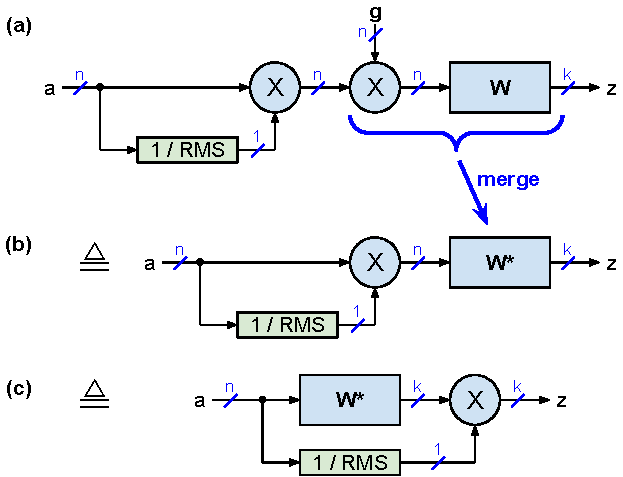
\includegraphics[scale=0.8]{../doc/fig/flashNorm_fig1.pdf}
  \caption{Mathematically identical implementations of RMSNorm followed by a linear layer.
    (a) Standard: normalization weights $\mathbf{g}$ are applied element-wise before $\mathbf{W}$.
    (b) Weightless: $\mathbf{g}$ is folded into $\mathbf{W}^* = \mathrm{diag}(\mathbf{g})\mathbf{W}$.
    (c) \textbf{FlashNorm}: normalization is also deferred to the output, enabling the GEMM
    ($\mathbf{W}^*$) and the RMS calculation to execute in parallel. $\triangleq$ denotes
    mathematical identity.}
\label{fig1} \end{figure}

\section{Introduction}
Normalization is indispensable to the training stability and generalization of
modern LLMs. RMSNorm~\citep{rms}, used by Llama~\citep{LLaMA},
Gemma~\citep{gemma}, Mistral~\citep{mistral}, and
OLMo~2~\citep{olmo2}, normalizes each activation vector by its root mean
square before scaling by learned weights. In the standard transformer network~\citep{vanilla},
RMSNorm is followed immediately by a linear (projection) layer---in both the attention and
feed-forward sub-networks of every transformer block.

This sequential structure conceals a hardware inefficiency. On processors with
dedicated vector units (for element-wise ops) and matrix units (for GEMMs), the
RMS value must be fully computed \emph{before} the linear layer can begin, because
the normalized activations are its input. The matrix unit therefore sits idle during
the RMS calculation---a bottleneck that compounds across all transformer layers and inference calls.

We address this bottleneck with \textbf{FlashNorm}, which makes two
mathematically equivalent transformations to the RMSNorm-then-linear pipeline shown in
Fig.~\ref{fig1}(a):

\begin{enumerate}
  \item \textbf{Weightless normalization.} The per-channel normalization weights
        $g_i$ are absorbed into the weight matrix of the following linear layer,
        eliminating them as a separate parameter tensor as illustrated in Fig.~\ref{fig1}(b).
  \item \textbf{Deferred normalization.} Because scaling by $1/\mathrm{RMS}(\mathbf{a})$
        commutes with matrix multiplication, the scalar normalization is
        moved to the \emph{output} of the linear layer as shown in Fig.~\ref{fig1}(c).
        This allows the GEMM and the RMS calculation to execute in parallel on separate
        hardware units.
\end{enumerate}

The name is inspired by FlashAttention \citep{flash-attention}, where the
softmax denominator is similarly deferred past a matrix multiplication to enable
parallel processing of keys and values.

FlashNorm requires no retraining, and weight folding can be applied post-hoc to any pretrained
checkpoint. We further show how the same ideas extend to Layer Normalization~\citep{layerNorm},
DyT~\citep{DyT}, GLU-variant FFNs~\citep{GLU}, RoPE-based attention~\citep{RoPE}, and
QK-normalization~\citep{QKnorm}.

\paragraph{Contributions.}
\begin{itemize}
  \item We formally characterize the commutativity of RMS normalization with
        bias-free matrix multiplication (Proposition~\ref{prop:commute}) and derive
        the exact conditions under which deferred normalization holds.
  \item We present FlashNorm as a unified framework covering RMSNorm, LayerNorm,
        DyT, GLU-FFNs, RoPE attention, and QK-norm.
  \item We provide a complete hardware timing analysis demonstrating the bottleneck
        that FlashNorm eliminates.
  \item We report controlled GPU benchmarks at two model scales and provide a
        reproducible Colab notebook alongside zero-loss weight-folding verification.
\end{itemize}

\section{Background and Related Work}

\paragraph{Normalization in transformers.}
Layer Normalization~\citep{layerNorm} applies mean centering followed by
variance normalization with learned scale and bias. RMSNorm~\citep{rms}
drops mean centering and bias, reducing to pure RMS-based scaling; it has become the
dominant normalization choice in recent open LLMs due to its simplicity and
comparable empirical performance. Dynamic Tanh (DyT)~\citep{DyT} is a
recently proposed drop-in replacement that eliminates the normalization computation
entirely, replacing it with a parameterized $\tanh$; FlashNorm is complementary in
that it targets the interaction between normalization and the subsequent linear layer.

\paragraph{Kernel fusion and operation reordering.}
Fusing small operations into a single GPU kernel is a standard optimization to
reduce memory bandwidth and kernel-launch overhead. \citet{openelm} report
that modifications to the layer normalization implementation significantly affect
tokens-per-second throughput, attributing this to a lack of kernel fusion. FlashNorm
reduces the number of kernel launches by eliminating the normalization weight
application as a separate step, and additionally enables parallelism between the
vector and matrix units that kernel fusion alone cannot achieve.

\paragraph{Weight folding and parameter elimination.}
The idea of absorbing one layer's parameters into a neighboring layer appears in
several forms. Batch normalization folding into convolutional weights is standard
practice in quantization-aware training and model deployment~\citep{quantJacob, convBN}.
PaLM~\citep{PaLM} removes bias parameters from all linear layers,
simplifying the computation graph. FlashNorm applies analogous reasoning to
normalization weights, showing that they are redundant given access to the subsequent
linear layer's weights.

\paragraph{FlashAttention.}
FlashAttention~\citep{flash-attention} is the closest conceptual predecessor:
it defers the softmax normalization (division by $\sum \exp$) past the multiplication
with the value matrix $V$, enabling online computation and improving memory
efficiency. FlashNorm applies the same reordering insight to the simpler setting of
RMS normalization and a dense linear layer.

\section{FlashNorm}
We now develop FlashNorm formally. All propositions assume bias-free linear layers
unless stated otherwise; Section~\ref{sec:bias} addresses the biased case.

\subsection{Weightless Normalization}
Let $\mathbf{a} \in \mathbb{R}^n$ be an activation vector. RMSNorm computes
\[
  \mathrm{RMSNorm}(\mathbf{a})_i = \frac{a_i}{\mathrm{RMS}(\mathbf{a})} \cdot g_i,
  \qquad
  \mathrm{RMS}(\mathbf{a}) = \sqrt{\frac{1}{n}\sum_{i=1}^n a_i^2},
\]
where $\mathbf{g} \in \mathbb{R}^n$ are learned normalization weights.
In transformer models, RMSNorm is followed by a linear layer $\mathbf{W} \in \mathbb{R}^{n \times k}$  as illustrated in Fig. \ref{fig1}(a):
\[
  \mathbf{z} = \mathrm{RMSNorm}(\mathbf{a})\, \mathbf{W}.
\]

\begin{proposition}[Weightless normalization]\label{prop:weightless}
Let $\mathbf{W}^* \in \mathbb{R}^{n \times k}$ be defined by $W^*_{i,j} = g_i \cdot W_{i,j}$.
Then $\mathbf{z} = \frac{\mathbf{a}}{\mathrm{RMS}(\mathbf{a})}\, \mathbf{W}^*$, i.e.,
the normalization weights $\mathbf{g}$ can be absorbed into $\mathbf{W}$ and need not
be stored or applied separately.
\end{proposition}

\begin{proof}
$z_j = \sum_i \frac{a_i}{\mathrm{RMS}(\mathbf{a})} g_i W_{i,j}
     = \sum_i \frac{a_i}{\mathrm{RMS}(\mathbf{a})} W^*_{i,j} $.
     % = \frac{1}{\mathrm{RMS}(\mathbf{a})} \sum_i a_i W^*_{i,j}
\end{proof}

This proposition holds for linear layers with or without a bias term at the output.
The practical implication is that the normalization weight vector $\mathbf{g}$ becomes
a redundant parameter: it can be folded into $\mathbf{W}$ once at load time, saving
memory, reducing the parameter count, and eliminating one vector-multiply kernel call
per forward pass.

\subsection{Deferred Normalization}

\begin{proposition}[Commutativity of RMS scaling with bias-free GEMM]\label{prop:commute}
Let $\mathbf{W}^*$ be as in Proposition~\ref{prop:weightless} and let the linear
layer be bias-free. Then
\[
  \mathbf{z}
  = \frac{\mathbf{a}}{\mathrm{RMS}(\mathbf{a})}\,\mathbf{W}^*
  = (\mathbf{a}\,\mathbf{W}^*)\cdot \frac{1}{\mathrm{RMS}(\mathbf{a})}.
\]
That is, the scalar normalization $1/\mathrm{RMS}(\mathbf{a})$ can be applied
\emph{after} the matrix multiplication.
\end{proposition}

\begin{proof}
Scalar multiplication commutes with matrix multiplication:
$(\alpha \mathbf{a})\mathbf{W}^* = (\mathbf{a}\mathbf{W}^*) \alpha$ for any scalar
$\alpha$. Setting $\alpha = 1/\mathrm{RMS}(\mathbf{a})$ gives the result.
\end{proof}

\begin{remark}[Bias case]
If the linear layer has a bias $\mathbf{c} \in \mathbb{R}^k$, deferred normalization
does not hold directly because
$(\mathbf{a}\mathbf{W}^* + \mathbf{c}) / \mathrm{RMS}(\mathbf{a}) \neq
 \mathbf{a}\mathbf{W}^*/\mathrm{RMS}(\mathbf{a}) + \mathbf{c}$.
In this case, Proposition~\ref{prop:weightless} (weightless normalization) still
applies, but the normalization must precede the bias addition.
\end{remark}

\begin{corollary}[Parallel execution]\label{cor:parallel}
Under the conditions of Proposition~\ref{prop:commute}, computing
$\mathbf{a}\mathbf{W}^*$ and $\mathrm{RMS}(\mathbf{a})$ are \emph{independent}
computations that may proceed in parallel. The final result requires only a single
vector-scalar multiply after both complete.
\end{corollary}

Figure~\ref{fig1} illustrates the three mathematically equivalent
implementations: (a) standard RMSNorm-then-linear, (b) weightless normalization,
and (c) the full FlashNorm with deferred normalization.

\subsection{Support for Normalization Bias}\label{sec:bias}
LayerNorm~\citep{layerNorm} and DyT~\citep{DyT} include an additive
bias $\boldsymbol{\beta}$ after scaling by $\mathbf{g}$. Fig. \ref{figA}
illustrates how this bias can be moved to
the output of the following linear layer, resulting in a modified bias
$\mathbf{c}^* = \mathbf{c} + \boldsymbol{\beta}\mathbf{W}$, see Fig. \ref{figA}(b).
After this elimination of $\boldsymbol{\beta}$, the normalization weights
$\mathbf{g}$ can be folded into the linear layer as per Proposition~\ref{prop:weightless}.
Note that deferred normalization (Proposition~\ref{prop:commute}) does not apply
once a bias is present; the scalar $1/\mathrm{RMS}(\mathbf{a})$ must be applied
before adding $\mathbf{c}^*$.

\begin{figure}[h!] \centering  % the [h!] tries to place the picture right here
  \includegraphics[scale=0.8]{../doc/fig/flashNorm_figA.pdf}
  \caption{Elimination of bias $\boldsymbol{\beta}$: (a) Before elimination with $\boldsymbol{\beta}$
    between normalization weights $\mathbf{g}$ and linear layer. (b) Optimized version with new
    bias term $\mathbf{c}^* = \mathbf{c} + \boldsymbol{\beta}\mathbf{W}$ at the output.}
\label{figA} \end{figure}

\subsection{Folding Mean Centering into a Preceding Linear Layer}
LayerNorm applies mean centering before RMSNorm. If mean centering is preceded by a
linear layer with weights $\mathbf{V} \in \mathbb{R}^{n \times n}$, the centering
can be absorbed into $\mathbf{V}$ without retraining.
Fig. \ref{figB}(a) shows the weight matrix $\mV$ followed by mean centering and RMSNorm.
\begin{figure}[h!] \centering  % the [h!] tries to place the picture right here
  \includegraphics[scale=0.8]{../doc/fig/flashNorm_figB.pdf}
  \caption{Elimination of mean centering: (a) Original weight matrix $\mV$ followed by mean centering. (b) Optimized version where the mean centering is merged into the modified weight matrix $\V*$.}
\label{figB} \end{figure}

The mean $\mu$ is calculated from the linear layer outputs $y_j$ as
$\mu = \frac{1}{n} \sum_{j=1}^n y_j$ where $y_j = \sum_{i=1}^n x_i V_{i,j}$.
Let $s_i = \sum_j V_{i,j}$ be the row sum of row $i$, then we can
calculate $\mu$ directly from the inputs $x_i$ as
\begin{equation*}
  \mu = \frac{1}{n} \sum_{j=1}^n \sum_{i=1}^n x_i V_{i,j} = \frac{1}{n} \sum_{i=1}^n x_i \left[ \sum_{j=1}^n V_{i,j} \right] = \frac{1}{n} \sum_{i=1}^n x_i s_i .
\end{equation*}
The mean-centered outputs are
\begin{equation*}
  a_j = y_j - \mu = \sum_{i=1}^n x_i V_{i,j} - \frac{1}{n} \sum_{i=1}^n x_i s_i
       = \sum_{i=1}^n x_i \underbrace{\left( V_{i,j} - \frac{s_i}{n} \right)}_{V^*_{i,j}},
\end{equation*}
so the modified weights $V^*_{i,j} = V_{i,j} - s_i/n$ absorb the mean centering
entirely, see Fig. \ref{figB}(b). This also provides a lossless recipe for converting a LayerNorm model
to RMSNorm without any retraining.

\section{Extensions}

\subsection{FlashNorm for FFNs with ReLU}
For bias-free FFNs with ReLU, the scale-invariance
$\mathrm{ReLU}(s \cdot \mathbf{a}) = s \cdot \mathrm{ReLU}(\mathbf{a})$ for $s \geq 0$ \citep{ReLU} allows
the RMS normalization to be deferred all the way to the FFN output, past both the up-projection
and the ReLU nonlinearity as illustrated in Fig. \ref{fig2}(b).
If the up-projection expands from $n$ to $f$ channels, this saves
$f - n$ multiply operations compared to applying the scaling at the FFN input.

\begin{figure}[h!] \centering
  \includegraphics[scale=0.8]{../doc/fig/flashNorm_fig2.pdf}
  \caption{FFN with ReLU and preceding flash normalization: (a) unoptimized version; (b) optimized version where the normalization is deferred to the output of the FFN. Up and Down denote the linear layers for up and down projections.}
\label{fig2} \end{figure}

\subsection{FlashNorm for FFNs with GLU Variants}
For GLU-variant FFNs~\citep{GLU}, the FlashNorm at the FFN
input requires scaling at both the Gate and Up projection outputs, see Fig. \ref{fig3}(a).
One of these scaling operations can be deferred to the FFN output, saving $f - n$ multiply operations
as shown in Fig. \ref{fig3}(b).
\begin{figure}[h!] \centering
  \includegraphics[scale=0.8]{../doc/fig/flashNorm_fig3.pdf}
  \caption{FFN with GLU variant and preceding flash normalization: (a) unoptimized version; (b) optimized version with fewer scaling multipliers.}
\label{fig3} \end{figure}

\paragraph{Special case: ReGLU and Bilinear GLU.}
When the activation function is ReLU (ReGLU) or linear (bilinear GLU) \citep{GLU}, both
scaling operations can be consolidated at the output as illustrated in Fig. \ref{fig4},
using the reciprocal of the \emph{squared} RMS (equivalently, the reciprocal of the mean square
$\mathrm{MS}(\mathbf{a})$:
\[
  \frac{1}{(\mathrm{RMS}(\mathbf{a}))^2}
  = \frac{1}{\mathrm{MS}(\mathbf{a})}
  = \frac{n}{\sum_{i=1}^n a_i^2}.
\]
\begin{figure}[h!] \centering
  \includegraphics[scale=0.8]{../doc/fig/flashNorm_fig4.pdf}
  \caption{FFN with ReGLU (or bilinear GLU) and preceding flash normalization: (a) unoptimized version;
    (b) optimized version, which saves $2f - n$ multiply operations.}
\label{fig4} \end{figure}

\subsection{FlashNorm for Attention with RoPE}
For the query ($\mathbf{Q}^*$) and key ($\mathbf{K}^*$) projections in RoPE-based
attention~\citep{RoPE}, the $1/\mathrm{RMS}(\mathbf{a})$ factor can be
fused with the precomputed RoPE cosine and sine tables, which are shared across
all attention heads as shown in Fig. \ref{fig5}.
Specifically, replacing $\cos(\cdot)$ with
$\cos(\cdot)/\mathrm{RMS}(\mathbf{a})$ (and similarly for $\sin$) eliminates the
per-head scaling entirely, saving $2hH - h$ multiply operations, where $h$ is the head
dimension and $H$ is the number of heads. Additionally, the $1/\sqrt{h}$ scaled
dot-product factor can be folded into the same scaling operation.
\begin{figure}[h!] \centering
  \includegraphics[scale=0.8]{../doc/fig/flashNorm_fig5.pdf}
  \caption{Flash normalization for scaled dot-product attention with RoPE: (a) unoptimized version; (b) optimized version where the normalization is fused with $\cosi$ and $\sini$.}
\label{fig5} \end{figure}

% OLD TEXT FOR Attention with RoPE
%Fig. \ref{fig5}(a) shows the Q and K linear layers with flash normalization followed by RoPE \citep{RoPE} and scaled dot-product attention \citep{vanilla}. More details on Figure \ref{fig5}:
%\begin{itemize}[topsep=-1pt]
%  \item Q* and K* are the linear layers for Q (queries) and K (keys) fused with the normalization weights of the activation vector $\a$ (according to flash normalization).
%  \item $h$ is the dimension of the attention heads.
%  \item The boxes labeled cos, sin, and RoPE perform $\vy = \vx \cdot \cosi + \text{permute}(\vx) \cdot \sini$, where
%  \begin{itemize}[topsep=-1pt]
%    \item $\text{permute}(\vx) = (-x_2, x_1, -x_4, x_3, \dots, -x_h, x_{h-1})$, see equation (34) of \citep{RoPE} for more details.
%    \item $\cosi = (\cos m \theta_1, \cos m \theta_1, \cos m \theta_2, \cos m \theta_2, \dots, \cos m \theta_{h/2}, \cos m \theta_{h/2})$ for position $m$.
%    \item $\sini = (\sin m \theta_1, \sin m \theta_1, \sin m \theta_2, \sin m \theta_2, \dots, \sin m \theta_{h/2}, \sin m \theta_{h/2})$ for position $m$.
%  \end{itemize}
%  \item Note that $\cosi$ and $\sini$ only depend on the position of activation vector $\a$ and are shared among all attention heads. Therefore, it’s more efficient to first scale $\cosi$ and $\sini$ by $1/ \rms$ as illustrated in Fig. \ref{fig5}(b). This saves $2hH - h$ multipliers, where $H$ is the number of attention heads.
%  \item Furthermore, we can fuse the scaling factor $1/ \sqrt{h}$ of the scaled dot-product with the $1/ \rms$ factor (note that we need to use $\sqrt{1/ \sqrt{h}}$ as a scaling factor for this).
%\end{itemize}

\subsection{QK-Normalization}\label{sec:qknorm}
Gemma~3~\citep{gemma3}, OLMo~2~\citep{olmo2}, OpenELM~\citep{openelm} and other LLMs
use per-head QK-normalization~\citep{QKnorm},
which applies RMSNorm to queries and keys \emph{after} the projection, preventing
direct application of FlashNorm. Two optimizations are still available:

\paragraph{Eliminating the pre-projection RMS.}
By the scale-invariance of RMS, $\mathrm{RMS}(s \cdot \mathbf{a}) = s \cdot \mathrm{RMS}(\mathbf{a})$.
When a FlashNorm RMS scaler $s_a$ is followed immediately by a QK-norm RMS scaler $s_c$ on the
projected output as shown in Fig. \ref{fig6} with activation vectors $\mathbf{a, b, c}$, the two scalers cancel:
$s_a \cdot s_c = s_a \cdot (s_b / s_a) = s_b$ because
$s_c = 1/\RMS{\mathbf{c}} = 1/\RMS{\mathbf{b} \cdot s_a} = 1/\left(s_a \cdot \RMS{\mathbf{b}}\right) = s_b / s_a$.
The pre-projection RMS calculation is therefore redundant and can be eliminated
as illustrated in Fig. \ref{fig6}(b).
The scale-invariance property of $\rms$ doesn’t hold exactly true for RMS with epsilon
(see appendix). This should not matter because the epsilon only makes an impact if the
RMS (or energy) of the activation vector is very small, in which case the epsilon limits
the up-scaling of this low-energy activation vector.

\begin{figure}[h!] \centering
  \includegraphics[scale=0.8]{../doc/fig/flashNorm_fig6.pdf}
  \caption{Linear layer with flash normalization followed by a second normalization: (a) unoptimized version; (b) optimized version.}
\label{fig6} \end{figure}

% OLD TEXT WITH MORE DETAILS
%Fig. \ref{fig6}(b) takes advantage of this property. We can express this
%by using the vectors $\a, \b, \c$ along the datapath in Fig. \ref{fig6} as follows:
%\begin{itemize}[topsep=-1pt]
%  \item Note that $s_c = \frac{1}{\RMS{\c}} = \frac{1}{\RMS{\b \cdot s_a}} = \frac{1}{s_a \cdot \RMS{\b}} = \frac{s_b}{s_a}$.
%  \item With above, we can show that the $y$ outputs of figures \ref{fig6}(a) and \ref{fig6}(b) are identical:
%    \begin{equation*}
%      y = \a \cdot \W* \cdot s_a \cdot s_c \cdot \vg = \a \cdot \W* \cdot s_a \cdot \frac{s_b}{s_a} \cdot \vg
%      = \a \cdot \W* \cdot s_b \cdot \vg
%    \end{equation*}
%\end{itemize}

\paragraph{Fusing QK-norm weights with RoPE.}
If QK-norm weights are shared across all heads of a layer (as in Gemma~3 and
OpenELM), they can be fused with the RoPE cosine and sine vectors, which are
already shared across heads, see Fig. \ref{fig7}.
The fused tables are computed once per layer, and
the normalization weights require only a permutation to align with RoPE's
interleaved layout: $\mathrm{permute}(\mathbf{g}) = (g_2, g_1, g_4, g_3, \ldots, g_h, g_{h-1})$.
\begin{figure}[h!] \centering
  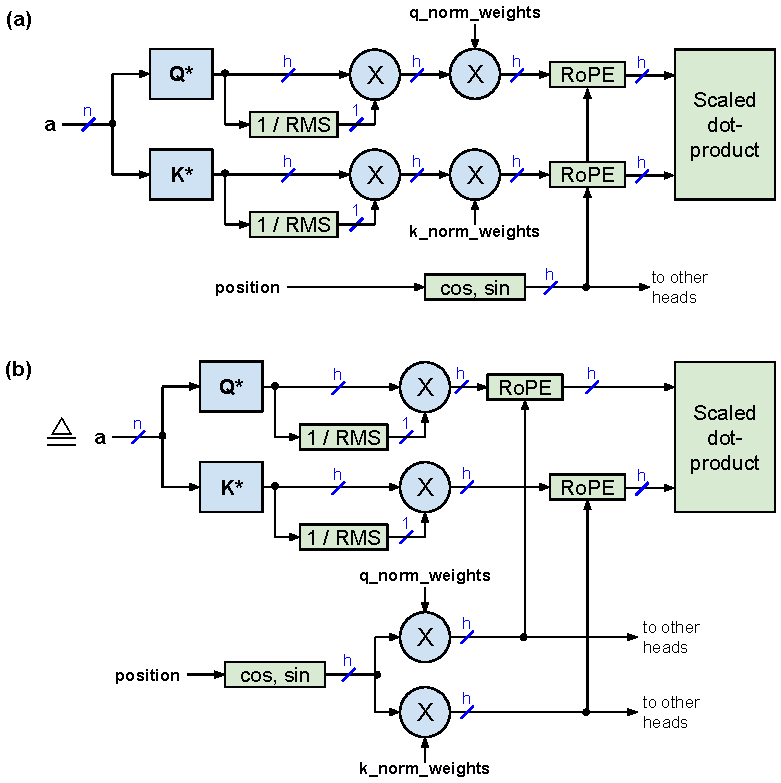
\includegraphics[scale=0.8]{../doc/fig/flashNorm_fig7.pdf}
  \caption{QK-norm with RoPE: (a) unoptimized version; (b) optimized version.}
\label{fig7} \end{figure}

% MORE DETAILS:
%This requires permutation of the normalization weights $\vg$ so that the boxes labeled cos, sin, and RoPE in Fig. \ref{fig7}(b) perform $\vy = \vx \cdot \left( \cosi \cdot \vg \right) + \text{permute}(\vx) \cdot \left( \sini \cdot \text{permuteg}(\vg) \right)$, where $\text{permuteg}(\vg) = (g_2, g_1, g_4, g_3, \dots, g_h, g_{h-1})$. For simplicity, Fig. \ref{fig7}(b) doesn't show the permutation of the normalization weights.

\section{Hardware Analysis}
We analyze the compute bottleneck that FlashNorm eliminates.
Consider a processor with one vector unit
(throughput: $m$ ops/cycle) and one matrix unit (throughput: $m^2$ ops/cycle) where $m$ is the processor width. Specifically:
\begin{itemize}
    \item Multiplying an $n$-vector with an $n \times n$ matrix takes $n^2$ MAD (multiply-add)
          operations, which takes $n^2/m^2$ matrix cycles.
    \item Computing  $1/\mathrm{RMS}(\mathbf{a})$ requires $n$ MAD operations (for squaring and adding)
          plus 2 scalar ops (for $\sqrt{n/x}$), which takes $n/m$ vector cycles if we ignore
          the 2 scalar ops.
    \item Scaling an $n$-vector by a scalar takes $n/m$ vector cycles.
\end{itemize}

Fig.~\ref{fig8} shows timing diagrams for the example $n = 512$ and $m = 128$.
Without FlashNorm (sequential execution), the matrix unit cannot begin until both
the RMS and the scaling are complete, imposing an 8 cycle bubble as shown in Fig.~\ref{fig8}(a).
The subsequent vector-matrix multiply takes $(512)^2 / (128)^2 = 16$ cycles; the total is 24 cycles.

With row-major ordering, the first rows of $\mathbf{W}^*$ can be processed
while later rows of the RMS accumulation are still in flight, reducing the bubble
to 5 cycles (total: 21 cycles), but the bottleneck persists, see Fig.~\ref{fig8}(b).

With FlashNorm (deferred normalization), the vector-matrix multiply ($\mathbf{a}\mathbf{W}^*$) and
the RMS calculation proceed fully in parallel on separate units as shown in Fig.~\ref{fig8}(c).
The scaling at the end can be performed in parallel to the matrix unit if $\mat{W}^*$ is processed in column-major order.
Total execution: 17 cycles---a \textbf{29\% reduction} versus the sequential baseline.
\begin{figure}[h!] \centering
  \includegraphics[scale=0.8]{../doc/fig/flashNorm_fig8.pdf}
  \caption{Timing diagrams for $n = 512, m = 128$.
    (a) Sequential: matrix unit idles 8 cycles.
    (b) Partial overlap with interleaved scaling and vector-matrix multiplication.
    (c) \textbf{FlashNorm}: vector-matrix multiply and RMS run fully in parallel; 17 cycles total, a
    29\% reduction over (a).}
\label{fig8} \end{figure}

% OLD, more details:
%\begin{itemize}[topsep=-1pt]
%  \item The matrix multiplications of the linear layers are performed by the matrix unit,
%        while the vector unit performs vector-wise operations such as RMSNorm and FlashNorm.
%  \item Let’s assume that the vector unit can perform $m$ operations per cycle and the matrix
%        unit can perform $m^2$ operations per cycle, where $m$ is the processor width. Specifically:
%  \begin{itemize}[topsep=-1pt]
%    \item Multiplying an $n$-element vector with an $n \times n$ matrix takes $n^2$ MAD (multiply-add)
%          operations, which takes $n^2/m^2$ cycles with our matrix unit.
%    \item Calculating $1/\rms$ takes $n$ MAD operations (for squaring and adding) plus 2 scalar
%          operations (for $\sqrt{n/x}$), which takes $n/m$ cycles with our vector unit if we ignore
%          the 2 scalar operations.
%    \item Scaling an $n$-element vector by a scaling factor takes $n$ multiply operations,
%          which takes $n/m$ cycles.
%  \end{itemize}
%\end{itemize}

\section{Experiments and conclusions}
Refer to \citep{hfFlashNorm, tricks} for Python code that demonstrates the mathematical equivalency of the optimizations presented in this paper. A reproducible Colab notebook for the GPU benchmarks below is available in the \verb+transformer-tricks+ repository\footnote{\url{https://github.com/OpenMachine-ai/transformer-tricks/blob/main/notebooks/flashNorm\_gpu\_benchmark.ipynb}}.

We verified lossless weight folding on SmolLM2-135M \citep{smollm} using \verb+flashify_repo()+ from the \verb+transformer-tricks+ package \citep{tricks}. The original and weight-folded models produce identical logits (max difference = 0.0, cosine similarity = 1.0) and identical generated text.

To validate the parallel execution described in Fig.~\ref{fig8}, we benchmarked the norm-then-project operation on an NVIDIA T4 GPU (65~TFLOPS FP16, 320~GB/s). We compare sequential execution (RMSNorm $\rightarrow$ GEMM) against FlashNorm with adaptive dispatch: when the GEMM is compute-bound (many tokens), the GEMM runs on tensor cores and $1/\rms$ runs on vector cores in parallel via separate CUDA streams; when memory-bound (few tokens), FlashNorm falls back to sequential execution to avoid stream overhead. Table~\ref{tab:overlap} shows the results at SmolLM2-135M scale, and Table~\ref{tab:overlap7b} at Llama-7B scale.

\begin{table}[h!] \centering
\caption{Norm+project latency on T4 GPU at SmolLM2-135M scale ($n{=}576, k{=}960$). Below the compute-bound threshold, FlashNorm falls back to sequential execution (0\% overhead).}
\label{tab:overlap}
\begin{tabular}{r r r r l}
\hline
Tokens & Sequential & FlashNorm & Speedup & Path \\
\hline
1      & 0.374\,ms & 0.374\,ms & $0.0$\% & sequential (fallback) \\
64     & 0.506\,ms & 0.506\,ms & $0.0$\% & sequential (fallback) \\
4096   & 0.704\,ms & 0.468\,ms & $+$33.6\% & parallel (overlap) \\
8192   & 0.929\,ms & 0.599\,ms & $+$35.5\% & parallel (overlap) \\
\hline
\end{tabular}
\end{table}

\begin{table}[h!] \centering
\caption{Norm+project latency on T4 GPU at Llama-7B scale ($n{=}4096, k{=}4096$).}
\label{tab:overlap7b}
\begin{tabular}{r r r r l}
\hline
Tokens & Sequential & FlashNorm & Speedup & Path \\
\hline
1      & 0.641\,ms & 0.641\,ms & $0.0$\% & sequential (fallback) \\
64     & 0.307\,ms & 0.307\,ms & $0.0$\% & sequential (fallback) \\
256    & 0.577\,ms & 0.577\,ms & $0.0$\% & sequential (fallback) \\
1024   & 1.882\,ms & 1.654\,ms & $+$12.1\% & parallel (overlap) \\
4096   & 7.628\,ms & 6.570\,ms & $+$13.9\% & parallel (overlap) \\
\hline
\end{tabular}
\end{table}

FlashNorm uses adaptive dispatch: the parallel path is used only when the GEMM is compute-bound (token count exceeds a hardware-dependent threshold). For memory-bound workloads such as autoregressive decoding, FlashNorm falls back to sequential execution (0\% overhead). This is because managing parallel CUDA streams introduces scheduling overhead that exceeds the time saved when the GEMM is small. Profiling individual operations within a SmolLM2-135M decoder layer at 4096 tokens confirms that the $1/\rms$ calculation takes ${\sim}0.08$\,ms per layer. Across 30 layers, the theoretical maximum savings from perfect overlap is ${\sim}5$\,ms out of ${\sim}60$\,ms total (${\sim}8\%$).

While the speedup on the norm+project operation itself is significant (33--35\%), the end-to-end model speedup is modest because this operation is a fraction of total layer time. For comparison, we measured a throughput of 204 tokens per second for OpenELM-270M with 4-bit weight quantization using the MLX framework on an M1 MacBook Air. This throughput increases to only 225 tokens per second when we remove RMSNorm entirely, giving an upper bound of $\leq$ 10\% for this model. Native integration into inference frameworks at the kernel level---where stream management overhead is negligible---would allow the 33--35\% operation-level improvement to translate more directly into end-to-end gains, particularly for larger models with bigger GEMMs.

For many applications, the main advantage of FlashNorm is simplification. This is similar to the simplifications we get from using RMSNorm over Layer Normalization (LayerNorm \citep{layerNorm}), and from PaLM's removal of bias-parameters from all linear layers \citep{PaLM}.

Future work includes integrating FlashNorm into popular frameworks such as HuggingFace Transformers \citep{HFtransformers}, whisper.cpp \citep{whisper-cpp}, llama.cpp \citep{llama-cpp}, vLLM \citep{vLLM}, llamafile \citep{llamafile}, LM Studio \citep{lmstudio}, Ollama \citep{ollama}, SGLang \citep{sglang}, and combining it with parameter quantization.

\section*{Acknowledgments}
We would like to thank Dmitry Belenko for helpful feedback on this work.

\appendix

\section{RMS with epsilon}
Many implementations add a small epsilon $\epsilon$ to the RMS value to limit the resulting scaling factor $1/\rms$ and to avoid division by zero as follows:
\begin{equation*}
 \text{RMSe}(\a) = \sqrt{\epsilon + \f1n \sas} = \sqrt{\epsilon + \left( \rms \right)^2}
\end{equation*}

$\text{RMSe}(\a)$ can be used as a drop-in-replacement for RMS. The popular HuggingFace transformer library calls this epsilon \verb+rms_norm_eps+, which is set to $10^{-5}$ for Llama3.

\section{Eliminating $1/n$}
This section details a small optimization that eliminates the constant term $1/n$ from the RMS calculation. First, we factor out $1/n$ as follows:
\begin{equation*}
  \rms = \sqrt{\f1n \sas} = \sqrt{\f1n} \sqrt{\sas} = \sqrt{\f1n} \cdot \text{RSS}(\a)
\end{equation*}
where $\text{RSS}(\a) = \sqrt{\sas}$. We can now merge the constant term into the normalization weights $g_i$ as follows:
\begin{equation*}
  y_i = \frac{a_i}{\rms} \cdot g_i =
  \frac{a_i}{\text{RSS}(\a)} \sqrt{n} \cdot g_i =
  \frac{a_i}{\text{RSS}(\a)}          \cdot g_i^\ast
\end{equation*}
with new normalization weights $g_i^\ast = \sqrt{n} \cdot g_i$ . These new normalization weights can now be merged with the weights $\mat{W}$ of the following linear layer as shown in the previous sections. This optimization also applies for the case where we add an epsilon as detailed in the previous section. In this case, we factor out $1/n$ as follows:
\begin{equation*}
  \text{RMSe}(\a) = \sqrt{\epsilon + \f1n \sas}
  = \sqrt{\f1n \left( n \epsilon + \sas \right)}
  %= \sqrt{\f1n} \sqrt{n \epsilon + \sas}
  = \sqrt{\f1n} \cdot \text{RSSe}(\a)
\end{equation*}
where $\text{RSSe}(\a) = \sqrt{n \epsilon + \sas}$.

\bibliographystyle{unsrtnat}
\bibliography{references}

\end{document}
